\documentclass[12pt]{article}
\pagestyle{fancy}
\usepackage{graphicx}
\usepackage{moresize}
%------------------------------------Document start-------------------------------------------%

\begin{document}

%------------------------------------titlepage-------------------------------------------%
 
\begin{titlepage}
\begin{center}
\newcommand {\HRule}{\rule{\linewidth}{0.5mm}}
\HRule\\[0.0cm]
\HUGE \bf{LibreHatti}\\[0.0cm]
\HRule\\
\Large{A Synopsis for six month training project}\\[0.4cm]
 \large{Master of Computer Applications}\\[0.4cm]
 \small{Batch(2013-2016)\\[0.5cm]

\includegraphics{images/gne.jpg}\\[0.5cm]


\begin{minipage}{0.4\textwidth}
\begin{flushleft} \large
{Submitted To:}\\
\textnormal{Prof. Inderjeet Singh.\\
M.C.A Deptt.} 
\end{flushleft}
\end{minipage}
~
\begin{minipage}{0.4\textwidth}
\begin{flushright} \large
{Submitted By:} \\
\textnormal{Manpreet kaur. \\
1311515.\\
Harmanjot Singh\\
1311507.\\
Monisha\\
1311518.\\
}
\end{flushright}
\end{minipage}\\[2cm]
 \large{Guru Nanak Dev Engineering College, Ludhiana.}\\[0.2cm]
\footnotesize{(A Autonomous College u/s 2(f) and 12(B) of UGC Act 1956.)}


\end{center}
\end{titlepage}
%------------------------------------titlepage end-------------------------------------------%

\newpage

%---------------------------table_of_contents generated automatically -----------------------%

\tableofcontents
\newpage

%------------------------------------Introduction to organisation-----------------------------------%

\section{Introduction to Organisation}
I had my Six Months Insdustrial Training at {\bf Testing And Consultancy Cell, GNDEC Ludhiana} under the guidance of Dr. H.S.Rai (Dean Testing & Consultancy Cell).Testing and Consultancy Cell was established in the year 1979 with a basic aim to produce quality service for technical problems at reasonable and affordable rates as a service to society in general and Engineering fraternity in particular. \par
   Consultancy Services are being rendered by various Departments of the College to the industry,
Sate Government Departments and Entrepreneurs and are extended in the form of expert advice
in design, testing of materials & equipment, technical surveys, technical audit, calibration of
instruments, preparation of technical feasibility reports etc. Consultancy projects of over Rs. 1.36
crores are completed by the Consultancy Cell during financial year 2011-12.
\newpage

%---------------------------------Introduction of Librehatti---------------------------------------%

\section{Introduction to LibreHatti}
Automation is the use of machines, control systems and information technologies to optimize pro-
ductivity of goods and delivery of services.\\ 
Automation is all about using the computer to:\\

%---------------------------------ordered list-----------------------------------------------------%

\begin{itemize}
\item Make your work less tedious.
\item Trim hours of your workload.
\item Reduce repetitive keyboard strokes or mouse-clicks.
\item Make data entry easier with fewer tabs or mouse movements.
\end{itemize}
The use of computer systems to execute a variety of office operations, such as word processing,
accounting, and e-mail refers to what we call automation.Automation helps in optimizing or au-
tomating existing office procedures.\par
LibreHatti is intended to provide elements which make it possible to simplify, improve, and
automate the activities involved in management and running of a company or a group of people.
It provides solutions to help clients improve internal processes, save money and deliver results.That is 'ingenuity to work'.
\subsection{Users of System}

%------------------------------------ordered lost-------------------------------------------------%

\begin{enumerate}
\item Administrator : Administrator can add or update (activate/inactivate) the details, and
also can see information of all employees. New categories and products can be added
or the existing can also be updated.
\item  Employee : As employees are directly related to clients, so they are able to add or
update the details of clients using this section. Administrator can see all the clients.
Employees can manage their clients only, and particular client can see his or her detail.
\item  Client : Clients are the end users that benefit from the this software. A client can get
information of all services available, and thus can apply for same. They can also view
the status of the number of the previous jobs done by them in the organisation.
\end{enumerate}
\subsection{Functional Requirements}
\textbf { Specific Requirements}: This phase covers the whole requirements for the system. After
understanding the system we need the input data to the system then we examine the output
and determine whether the output from the system is according to our requirements or not.
This phase also describe the software and non-functional requirements of the system.\\ 

%------------------------------------ordered list-------------------------------------------------%

\subsubsection {Input Requirements}
\begin{enumerate}
\item Client Details
\item  Order Details
\item  Extra Charges Details
\item  Categories and products Details
\item  Organisation & Department Details
\item  Rate List
\item  Staff Details
\end{enumerate}
\subsubsection{Output Requirements}
\begin{enumerate}
\item Interface for administrator to configure the system.
\item  Listing of all the services offered.
\item  Interface for clients and employees.
\item  Automatic generation of Reports, Bills, Receipts, and Vouchers for clients.
\item  Calculation of order amount.
\end{enumerate}
\subsubsection{Software Requirements}
\begin{enumerate}
\item rogramming language: Python 2.7+
\item  Framework: Django 1.7
\item  Web Languages: Html, Java Script, CSS
\item  Database: MySQL Database Server 5.1
\item Text editor: vi, vim, gedit
\item Operating System:Ubuntu 14.04 LTS
\item Server: Apache2
\end{enumerate}
\subsubsection {Hardware Requirements(Deploymentserver)}
\begin{itemize}
\item Operating system: Ubuntu 14.04 LTS.
\item Processor: Intel Pentinum Processor 4, 2.4GHZ or equivalent.
\item RAM: 1GB.
\item HDD:80 GB.
\end{itemize} 
\subsubsection{Hardware Requirements(End User's PC)}
  \begin{itemize}
  \item Operating system: Ubuntu 14.04 LTS.
  \item Processor: Intel Pentinum Processor , 233 MHZ or equivalent.
  \item RAM: 1GB.
  \item HDD:100 MB of free HDD space for internet cache.
  \end{itemize}

\subsection{Non-Functional Requirements}
\begin{enumerate}
\item Usability: Simple user interfaces that a layman can understand.
\item  Speed: Speed of the system should be responDsive i.e. Response to a particular action should
be available in short period of time. For e.g., Updating the project tasks take few seconds
for the changes if the entry is not starred.

%------------------------------------------System Design------------------------------------%

\section{System Design}
System design is the process or art of defining the architecture, components, modules, interfaces,
and data for a system to satisfy specified requirements. One could see it as the application of
systems theory to product development.System design include External design, In Logical design and Physical design.\\
\subsection{Design Notations}
Data Flow Diagrams:


\begin{figure}[!h]
 \centering
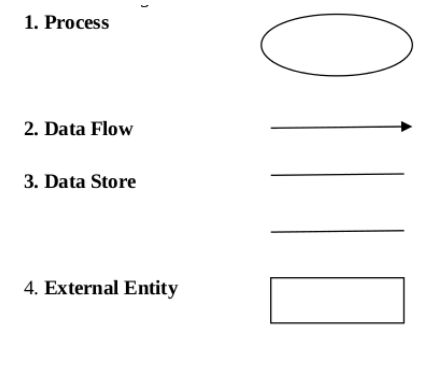
\includegraphics[scale=0.50]{images/diag.png}
\caption{Data Flow Diagram}
\end{figure}
Flow Chart:\\[0.5cm]
\begin{figure}[!h]
\centering
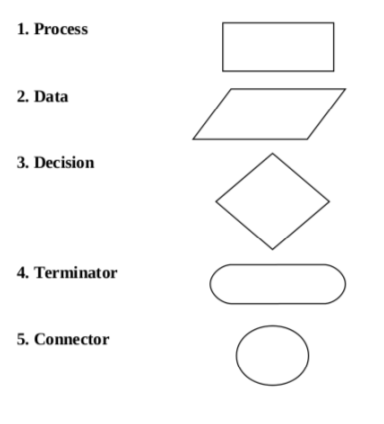
\includegraphics[scale=0.50]{images/flowc.png}
\caption{Flow Chart}
\end{figure}

\newpage
\subsection{Data Flow Diagrams}
\subsubsection{level 0}
\subsubsection{level 1}
\begin{figure}[!h]
\centering
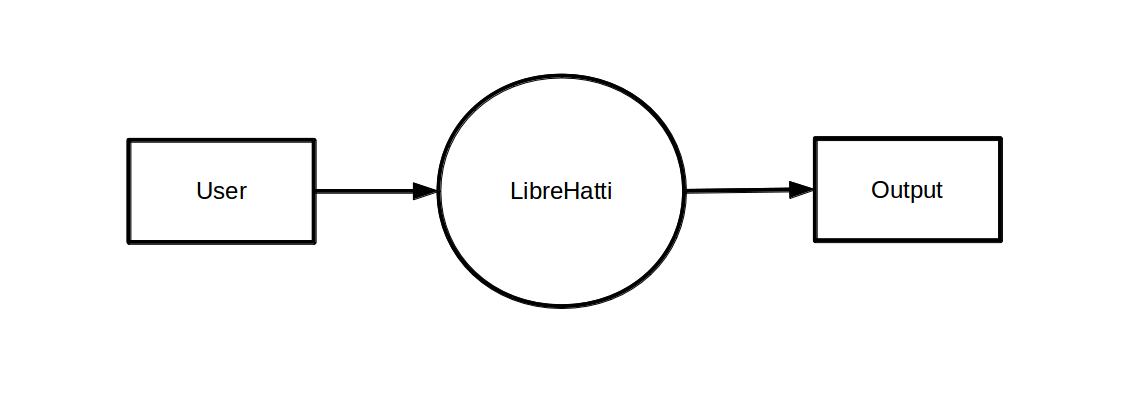
\includegraphics[width=120mm]{images/level0.png}
\caption{level0}
\end{figure}


\begin{figure}[!h]
\centering
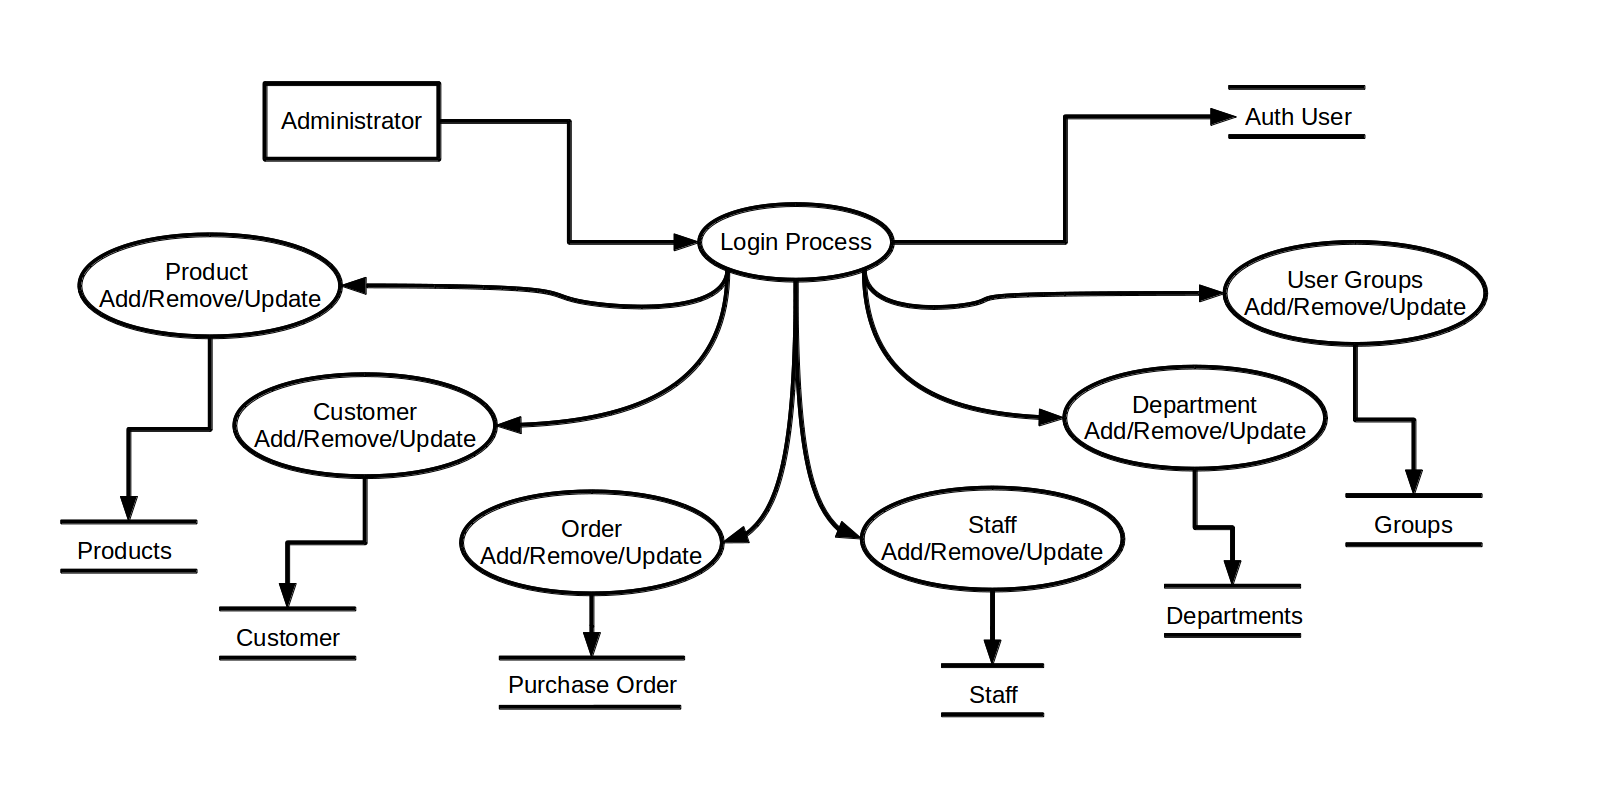
\includegraphics[width=130mm]{images/level1.png}
\caption{level 1}
\end{figure} 
\subsection{Database Design}
The Database of LibreHatti contains various tables according to requirements.
\section{Methologies used }
\subsection{EAV}
Entity-attribute-value model (EAV) is a data model to describe entities where the number of attributes (properties, parameters) that can be used to describe them is potentially vast, but the number that will actually apply to a given entity is relatively modest. EAV is also known as object-attribute-value model, vertical database model and open schema.\\ \\
Data is recorded as three columns:
\begin{itemize}
\item The entity: the item being described.
\item  The attribute or parameter: a foreign key into a table of attribute definitions. At the
very least, the attribute definitions table would contain the following columns: an attribute
ID, attribute name, description, data type, and columns assisting input validation, e.g.,
maximum string length and regular expression, set of permissible values, etc.
\item  The value of the attribute.
\end{itemize}\\ 
In LibreHatti, there may be a number of products with a number of attributes. If we follow
the old normalised approach of storing these attributes for all the products, it will lead to a huge
database and an inefficient way to access values from the database. Using EAV only the required
attributes for products are stored and makes the system efficient though denormalised.

\subsection{MVC}
Model-view-controller (MVC) is a software architectural pattern for implementing user interfaces.
It divides a given software application into three interconnected parts, so as to separate internal
representations of information from the ways that information is presented to or accepted from
the user.\\ \\
The components are as follows:\\
\begin{enumerate}
\item The central component of MVC, the model, captures the behavior of the application in terms
of its problem domain, independent of the user interface. The model directly manages the
data, logic and rules of the application.
\item  A view can be any output representation of information, such as a chart or a diagram;
multiple views of the same information are possible, such as a bar chart for management and
a tabular view for accountants.
\item  The third part, the controller, accepts input and converts it to commands for the model or
view.
\end{enumerate}
\subsection{MPTT}
Modified Preorder Tree Traversal is a technique for storing hierarchical data in a database. The
aim is to make retrieval operations very efficient.
\subsection{Python}
Python is a server side language Which can be used with Django.
\subsection{Django}
Django is a framework which is used for creating web applications. Its framework devide all work in different different modules such as template files are separate, url files are separately placed.
\newpage

%----------------------------------------------Biblograpy----------------------------------------%

\section{Biblography}
\begin{itemize}
\item Dr. H.S Rai
\item Internet
\item Great Developers
\item Mentor
\end{itemize}
\end{document}

%---------------------------------------------End Document------------------------------------------%

